% arara: xelatex
% arara: xelatex
% arara: xelatex

% options:
% thesis=B bachelor's thesis
% thesis=M master's thesis
% czech thesis in Czech language
% english thesis in English language
% hidelinks remove colour boxes around hyperlinks

\documentclass[thesis=M,english]{FITthesis}[2012/10/20]

\usepackage[utf8]{inputenc}

\usepackage{graphicx} %graphics files inclusion
% \usepackage{subfig} %subfigures
% \usepackage{amsmath} %advanced maths
% \usepackage{amssymb} %additional math symbols

\usepackage{dirtree} %directory tree visualisation

% ADDED BY ME
\usepackage{blindtext} % lorem ipsum
\usepackage{todonotes} 

\newcommand{\todotext}[1]{\textcolor{red}{\textbf{[[#1]]}}}
\definecolor{mygray}{gray}{0.6}
\newcommand{\blind}[1][1]{\textcolor{mygray}{\Blindtext[#1][1]}}

\setlength{\fboxsep}{0.005pt}
\newcommand{\tmpframe}[1]{\fbox{#1}}
%\renewcommand{\tmpframe}[1]{#1}

% list of acronyms
% \usepackage[acronym,nonumberlist,toc,numberedsection=autolabel,nomain]{glossaries}
\iflanguage{czech}{\renewcommand*{\acronymname}{Seznam pou{\v z}it{\' y}ch zkratek}}{}
% \makeglossaries

\newcommand{\tg}{\mathop{\mathrm{tg}}} %cesky tangens
\newcommand{\cotg}{\mathop{\mathrm{cotg}}} %cesky cotangens

% % % % % % % % % % % % % % % % % % % % % % % % % % % % % % % % % % % 
% % % % % % % % % % % % % % % % % % % % % % % % % % % % % % % % % % % 
\department{Department of theoretical computer science}
\title{Contextual Shell History}
\authorGN{Šimon} %author's given name/names
\authorFN{Let} %author's surname
\authorWithDegrees{Bc. Šimon Let} %author's name with academic degrees
\author{Šimon Let} %author's name without academic degrees
\supervisor{Ing. Lukáš Bařinka}
% my BP thesis: I~would like to thank my supervisor Ing. V{\' i}t List{\' i}k, without his assistance and guidance this thesis would have not be accomplished.
% \par Then I~would like to thank Ing. Michal Bukovsk{\' y} along with his whole Email.cz team in Seznam.cz for letting me work with them and use their data.
% \par My thanks also goes to RNDr. Jana Strakov{\' a} at. el for developing Nametag, Named entity recognition solution, I~used in this thesis, and answering my questions.
% \par Finally I~want to thank my family and friends for their support trough my whole studies.
\acknowledgements{TODO: I would like to thank my supervisor Ing. Lukáš Bařinka for his guidance, my colleagues and friends for their feedback, hundreds of people who downloaded this project for their trust, and my family for support during writing this thesis. Installfest for accepting my talk about this project. Github users who submitted issues and pull requests to the project.}
\abstractCS{TODO: Tato práce se zabývá slovními slovníkovými metodami komprese dat, specifickou částí bezztrátových metod komprese dat. Součástí publikace jsou rovněž některé znakově orientované slovníkové metody, především z~rodiny LZ algoritmů, potřebné k~pochopení složitějších slovních metod. Stěžejní dílem práce je popis implementovaných algoritmů pro slovní slovníkovou kompresi dat, jejich modifikací a především výsledky provedených testů, stejně jako jejich vyhodnocení. V~publikaci jsou zároveň uvedeny detaily implementace aplikace a její uživatelská příručka.}
\abstractEN{TODO: This thesis is an enhancement for standard shell history. It records shell history with context. It uses the recorded context to make it easier to find relevant history records and to make it possible to search search history using context explicitly.


This thesis is concerned with word-based dictionary methods of data compression. The word-based dictionary methods are part of lossless data compression methods. The character-based dictionary compression methods, especially from LZ-algorithms family, are a part of this issue. These compression methods are very important to understand more difficult word-based ones. The main sight of this publication is description of implemented word-based dictionary compression algorithms. Modifications of these methods and results of experiments are included too. There are also details contextual with implementation of the application and its user manual. The objective of this thesis
is examination of word-based dictionary data compression methods, possibilities of their improvement and their implementation linked with experiments on well-known data compression corpuses.}
\placeForDeclarationOfAuthenticity{Prague} %where you have signed the declaration
\keywordsCS{Shell, Příkazová řádka, Historie shellu, Nástroje produktivity}
\keywordsEN{Shell, Command line, Shell history, Productivity tools}
\declarationOfAuthenticityOption{1} %select as appropriate, according to the desired license
% \website{https://github.com/curusarn/master-thesis} %optional URL (remove entirely if you have no URL for this thesis) TODO: put the thesis up

\begin{document}

% \newacronym{LZW}{LZW}{Lempel Ziv Welch}
% \newacronym{RLE}{RLE}{Run-Length Encoding}
\begin{introduction}

Dummy citation \cite{greenberg1993computer}

\todotext{TODO: explain what is this work about}

\todotext{TODO: argue why is this work important}

\blind[0]

\todotext{TODO: describe the contents of this work / layout}

\blind[2]

\end{introduction}


\chapter{Analysis}

\todotext{TODO: describe layout/contents of the chapter}

\blind

\section{Shells, existing shell history features and tools}

\todotext{TODO: describe contents of this section}

\blind

\subsection{Recurrent systems}

\blind

\subsection{Shells and built-in history features}

\todo{TODO: shell history configurations options}

\blind[4]

\todotext{TODO: short conclusion about shells}

\subsection{History features of Read-eval-print loops}

\blind[1]

\subsection{Existing history tools}

\blind[4]

\todotext{TODO: short conclusion about history tools}

\section{How people use shell and shell history}

\todotext{TODO: intro - why we analyze people}

\blind

\todotext{TODO: introduce personas}

\todotext{TODO: describe use cases}

\blind[2]

\subsection{How people use tools}

\blind[2]

\subsection{How people use shell}

\todotext{TODO: Greenberg conducted a study in his work \cite{greenberg1993computer} in 19XX which provides a lot of insight into how people use shell. It's not obvious that conclusions and ideas in the work still hold. To make sure that the usage of shell didn't change to the point where we can't use the ideas anymore. }

plots:

Figure 3.1. The normalized command frequency, compared with Zipf.

\begin{figure}
  \tmpframe{\includegraphics[width=\linewidth]{figures/greenberg/plot_ref_zipf-cmd-frq.png}}
  \caption{The normalized command frequency, compared with Zipf. (Greenberg)}
\end{figure}

\begin{figure}
  \tmpframe{\includegraphics[width=\linewidth]{figures/greenberg_new/plot_zipf-cmd-frq.png}}
  \caption{The normalized command frequency, compared with Zipf.}
\end{figure}


Figure 3.2. Command vocabulary size vs. the number of command
lines entered for four individuals.

\begin{figure}
  \tmpframe{\includegraphics[width=\linewidth]{figures/greenberg/plot_ref_cmd-vocab-size.png}}
  \caption{Command vocabulary size vs. the number of command
lines entered for four individuals. (Greenberg)}
\end{figure}

\begin{figure}
  \tmpframe{\includegraphics[width=\linewidth]{figures/greenberg_new/plot_cmd-vocab-size.png}}
  \caption{Command vocabulary size vs. the number of command
lines entered for four individuals.}
\end{figure}


Figure 3.3. Sequential structure of UNIX command usage, from Figure 4
in Hanson et al. (1984).

\begin{figure}
  \tmpframe{\includegraphics[width=\linewidth]{figures/greenberg/graph_ref_cmd-sequences.png}}
  \caption{Sequential structure of UNIX command usage, from Figure 4
in Hanson et al. (1984). (Greenberg)}
\end{figure}

\begin{figure}
  \tmpframe{\includegraphics[width=\linewidth]{figures/greenberg_new/graph_cmd-sequences.pdf}}
  \caption{Sequential structure of command usage.}
\end{figure}


Table 5.2. The average recurrence rate of the four sample UNIX user
groups



Figure 5.6. Command line vocabulary size vs. the number of commands
entered for four typical individuals.


\blind[4]

\subsection{How people use shell history}

\blind[4]


\todotext{TODO: conclusion of the chapter}

\blind

\section{Available contextual information}

\todotext{TODO: intro}

\subsection{Directly available contextual information}

\blind[2]

\subsection{Derivable contextual information}

\blind[2]

\todotext{TODO: conclusion of the section}



\chapter{Design}
\todotext{TODO: intro describe contents of the chapter}

\blind
\todo{order of design chapters can change}
\section{Recording contextual history}

\todotext{TODO: what to record}

\blind[2]

\section{Front-end and User interaction}\todo{I don't like the title}

\todotext{TODO: intro}

\blind

\subsection{Standard history features}

\todotext{TODO: describe why it's important to respect the standard history features}

\todotext{TODO: which history features are we keeping/enhancing/leaving intact}

\blind[3]

\todotext{TODO: conclusion for further design ?}



\subsection{Core ideas, principals, design decisions, and features}\todo{weird title}

\todotext{TODO: intro: ideas in this chapter are essential for this work / project}

\todotext{TODO: features of the project - weird todo}

\blind[3]

\subsection{Possible features}

\todotext{TODO: intro: this section describes features that were considered during the design - for each feature we evaluate how well it would fit with the rest of the design. Some of the features were explicitly suggested by users and some features are included for the sake of completeness (because they make sense).}

\todo{TODO: list the features}


\section{Back-end}\todo{I don't like the title}

\blind

\section{Testing the design}

\todotext{TODO: explain why we want to test the design - intro}

\todotext{TODO: principals, guidelines, etc. are we are using}

\blind[3]

\chapter{Implementation}
\todotext{describe layout/contents of the chapter}

\blind

\section{Daemon}\todo{do we need this or is introduction enough}

\blind

\section{Choosing Go}

\blind[3]

\section{Recording shell history with context}

\blind

\subsection{History format}

\todotext{NOTE: both on disk and in transfer}

\blind

\subsection{Shell integration and hooks}

\blind

\subsection{History record merging}

\blind

\section{Custom arrow key bindings}

\todotext{TODO: intro: we want arrow key bindings to be able to record usage related metadata + it's a good idea to have the option to customize and use context to enhance arrow key bindings. Plus impossibility of gathering usage data and using the default bindings (at least in bash)}

\blind

\subsection{Keybinding custom functions in zsh}

\blind

\subsection{Keybinding custom functions in bash}

\blind


\subsection{Universal keybinding library}
\todotext{TODO: explain why: as you see bash and zsh have a different ways of supporting custom keybindings. To simplify our codebase we extracted the keybind setting logic into a library. (unified way to set keybindings)}

\blind

\todo{? talk about performance, daemon, etc.}

\section{Fullscreen command line history searching application}

\todo{TODO: subsections}


\section{Daemon components}

\todotext{TODO: describe why we need components}

\begin{figure}
  \tmpframe{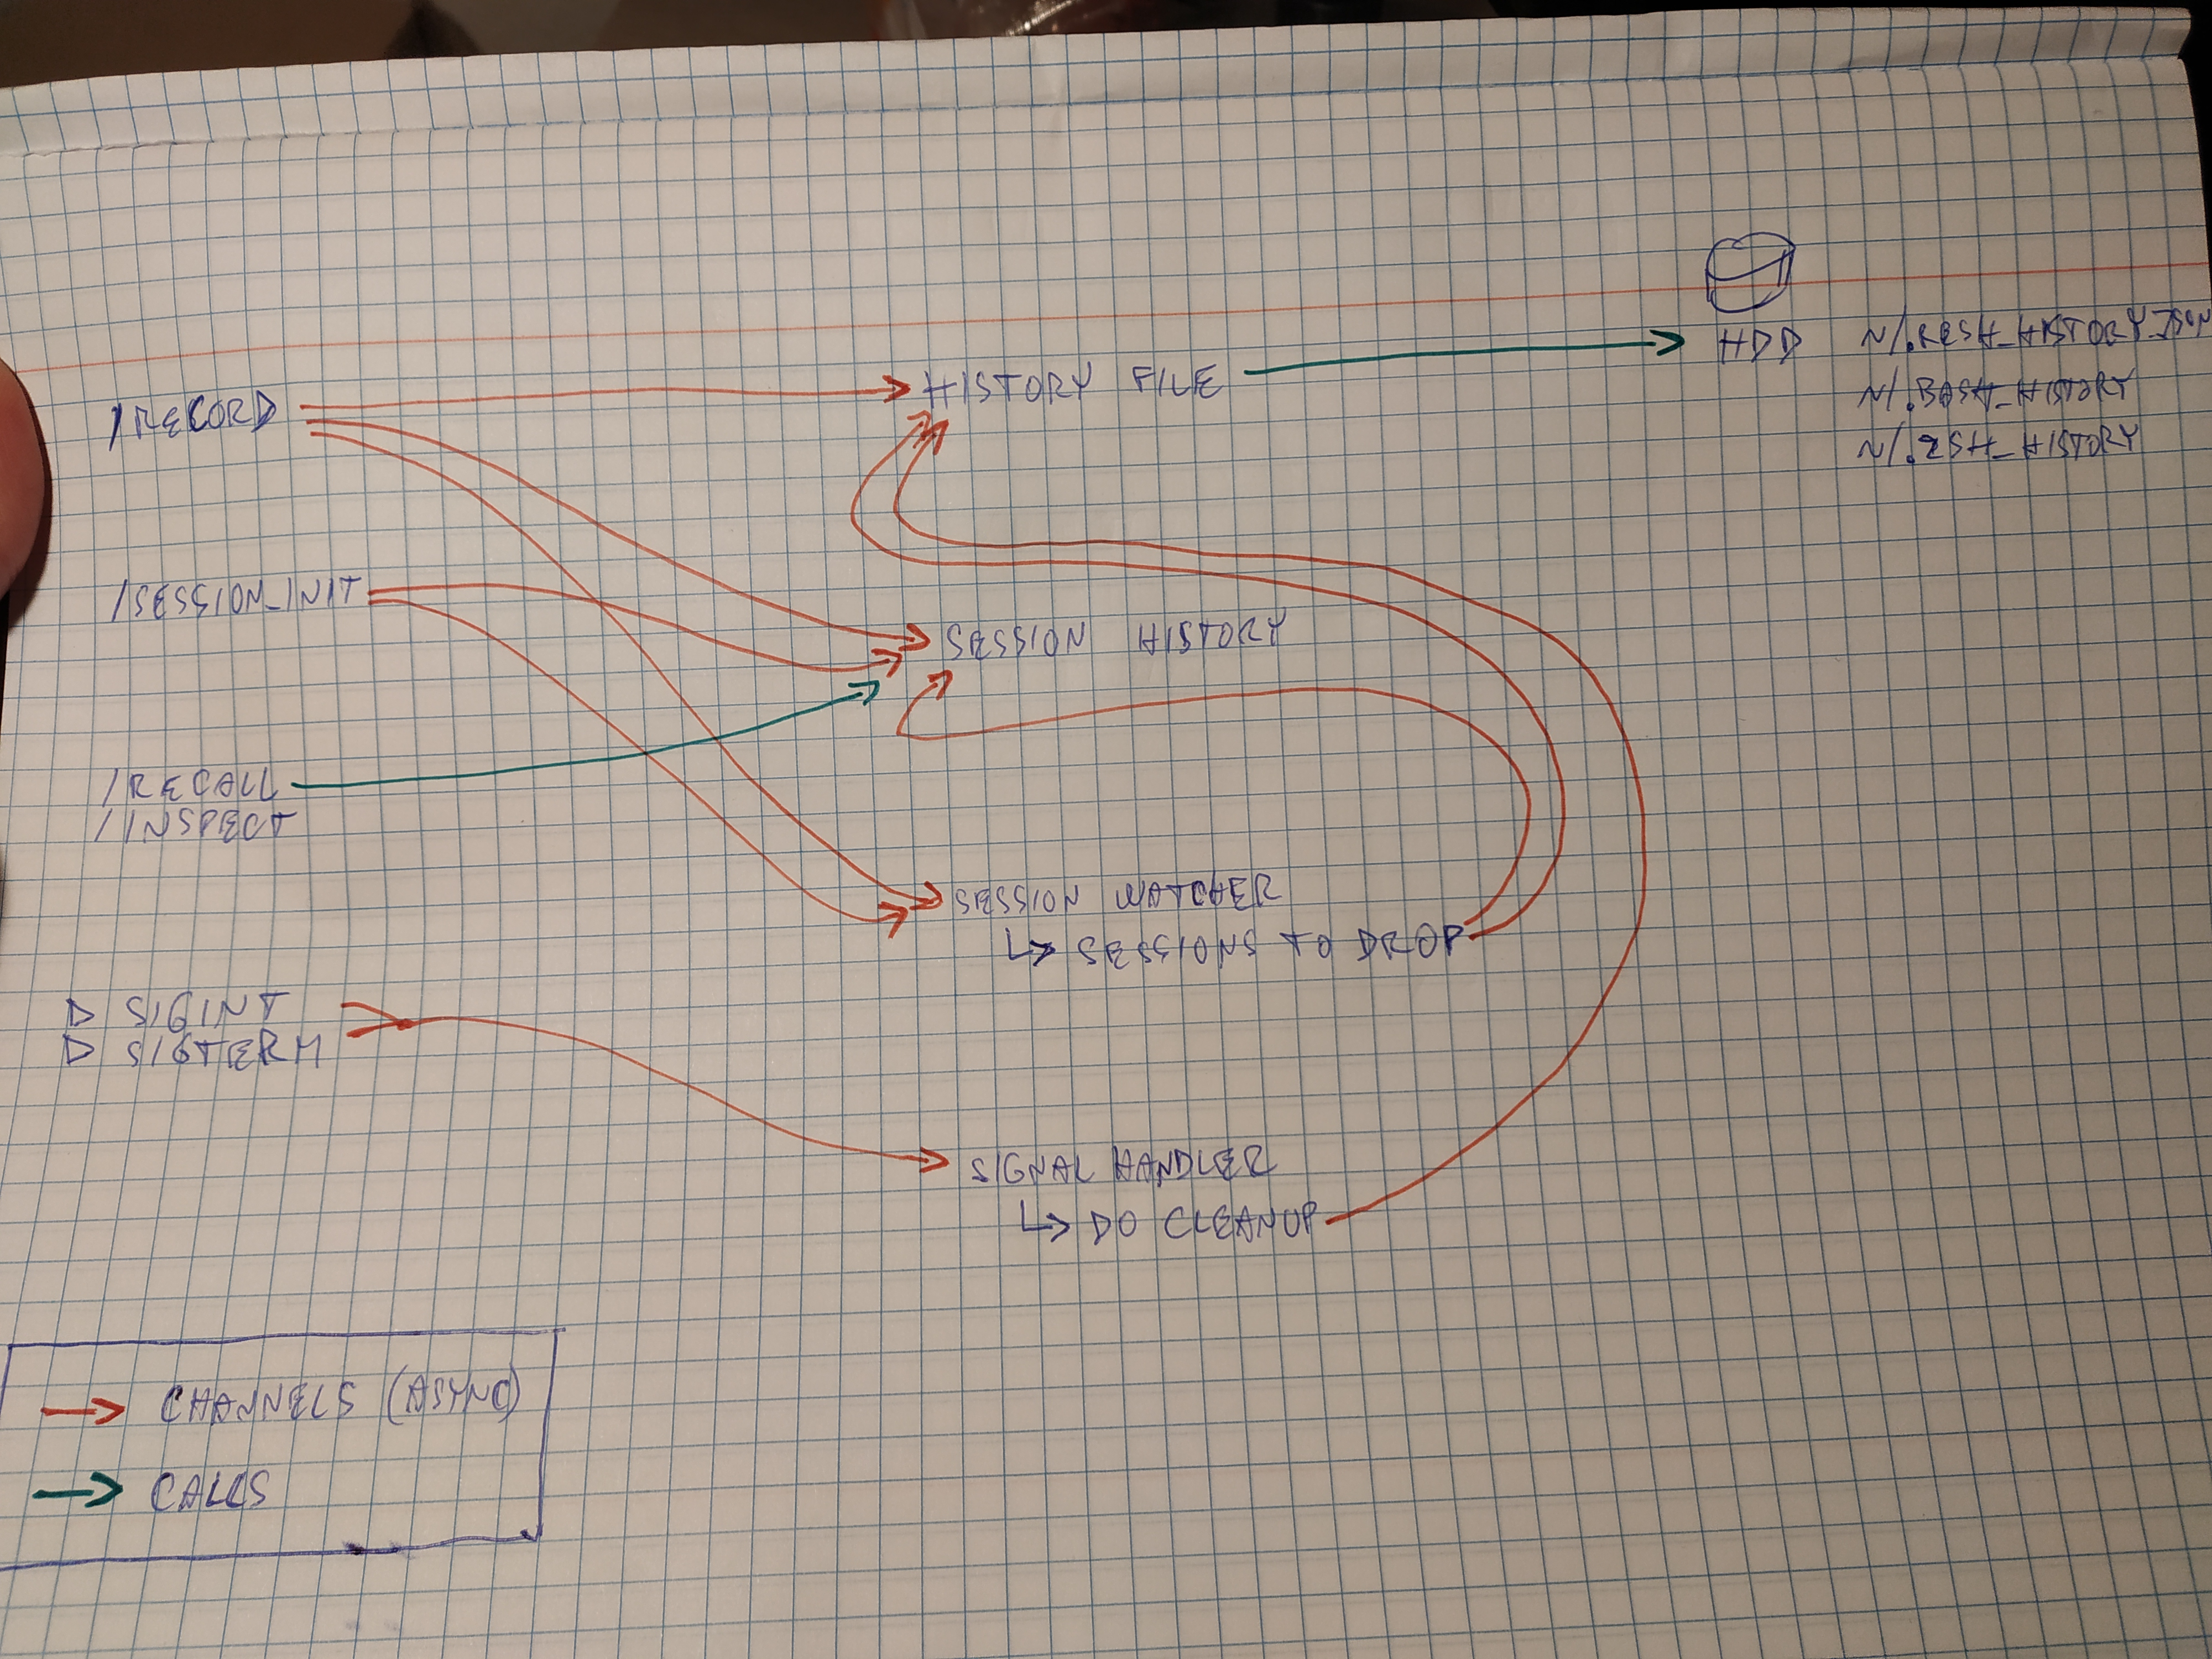
\includegraphics[width=\linewidth]{figures/daemon-components.jpg}}
  \caption{One image. \todotext{TODO: write a title}}
  \label{fig:TODO}
\end{figure}

\subsection{Server}

\subsection{History file}

\subsection{Session history}
\todotext{TODO: explain: there are implications for the daemon if we want responsive arrow key bindings}

\subsection{Expired session tracking}


\subsection{Signal handling}

\blind

\section{Control and configuration}

\blind

\section{Installation, updates, and build process}

\todotext{TODO: explain how simple the installation is. plus updates.}

\blind

\subsection{Installation and updates}
\todotext{TODO: explain how installation works}

\blind

\subsection{Production and development build process}
\todotext{TODO: explain the build process}

\blind[2]


\chapter{Testing and Evaluation}

\todotext{TODO: describe layout/contents of the chapter}

\todotext{TODO: describe how history tools can be usable}

\todotext{TODO: describe what influences usability of the tools}

\todotext{TODO: explain which parts of the system should be tested and why}

\blind[3]

\section{Metrics}

\todotext{TODO: describe why we use metrics}

\subsection{Metrics traditionally used to evaluate history tools}\todo{break down into more subsections ?}

\todotext{TODO: describe which metrics were used for history tools in the past}

\subsection{Newly suggested metrics}\todo{break down into more subsections ?}

\todotext{TODO: suggest new metrics + explain how they are better than the original ones}

\subsection{Evaluation using suggested metrics}

\todotext{TODO: explain used methods}

\todotext{TODO: use metrics to evaluate usefulness of the work}


\section{Use cases}



\begin{conclusion}

\end{conclusion}

\bibliographystyle{iso690.bst}
\bibliography{ref}

\appendix

% \printglossaries

\chapter{Contents of SD card}\label{app:SDcontent}

Visualise the contents of enclosed media. Use of \verb|dirtree| is recommended. Note that directories src and text with appropriate contents are mandatory.


\begin{figure}
	\dirtree{%
		.1 readme.txt\DTcomment{the file with CD contents description}.
		.1 data\DTcomment{the data files directory}.
		.2 graphs\DTcomment{the directory of graphs of experiments}.
		.3 *.eps\DTcomment{the B/W graphs}.
		.3 *.png\DTcomment{the color graphs}.
		.3 *.dat\DTcomment{the graphs data files}.
		.1 exe\DTcomment{the directory with executable WBDCM program}.
		.2 wbdcm\DTcomment{the WBDCM program executable (UNIX)}.
		.2 wbdcm.exe\DTcomment{the WBDCM program executable (Windows)}.
		.1 src\DTcomment{the directory of source codes}.
		.2 wbdcm\DTcomment{the directory of WBDCM program}.
		.3 Makefile\DTcomment{the makefile of WBDCM program (UNIX)}.
		.2 thesis\DTcomment{the directory of \LaTeX{} source codes of the thesis}.
		.3 figures\DTcomment{the thesis figures directory}.
		.3 *.tex\DTcomment{the \LaTeX{} source code files of the thesis}.
		.1 text\DTcomment{the thesis text directory}.
		.2 thesis.pdf\DTcomment{the Diploma thesis in PDF format}.
		.2 thesis.ps\DTcomment{the Diploma thesis in PS format}.
	}
\end{figure}


\end{document}
